
\section{Обзор предметной области} % (fold)
\label{sec:domain}

В данном разделе будет произведён обзор предметной области задачи, решаемой в рамках дипломного проекта;
% рассмотрены вопросы о сущности байесовых сетей и принципе их работы; приведена оценка сложности различных проблем, возникающих при применении вероятностных сетей для решения прикладных задач.
% Также будут рассмотрены принципы работы алгоритмов вывода структуры по данным, реализованных в программном обеспечении разработанном в рамках дипломного проекта, и произведено сравнение с существующим ПО для решения схожих задач.

\subsection{Предметная область}
\label{sub:domain:ip}
Объектом исследования данной работы является порядок купли-продажи жилых помещений, который регулирует вопрос прав человека на жилое помещение. Под предметом исследования понимаются современные проблемы регулирования продажи жилого помещения.

Следует отметить, что современный рынок жилья существенно отличается от рынка прошлых лет. Круг традиционных участников договора купли-продажи значительно расширился. Теперь обычно в сделку кроме покупателя и продавца включается третья сторона - посредник, в качестве которого выступает либо риэлтерская фирма, либо частный маклер. В сделках на рынке жилья все большую роль играют коммерческие банки, биржи, страховые компании, инвестиционные фонды и другие рыночные институты.

Учитывая высокую стоимость жилой площади, сумма заключаемых сделок оценивается в больших деньгах. Квартирный бизнес является одним из самых выгодных. Посреднические организации - риэлтерские фирмы и отдельные маклеры готовы оказать любые услуги гражданам по распоряжению принадлежащими им квартирами и домами, получая при этом наибольшие дивиденды.

К договору купли-продажи жилья применяются обязательные требования:

\begin{itemize}
	\item письменная форма в виде одного документа, подписанного сторонами, с государственной регистрацией сделки и нового собственника;
	\item указание имени и регистрации по месту жительства;
	\item определенная (однозначная) характеристика предмета сделки;
	\item данные о возможных правах третьих лиц;
	\item цена жилого помещения и оплата расходов по договору;
	\item срок и порядок передачи имущества.
	\item Покупатели квартир преследуют различные цели:
	\item улучшение жилищных условий;
	\item перемена места жительства;
	\item вложение капитала в недвижимость для последующей продажи и получения дохода.
\end{itemize}

Купля и продажа недвижимости включает в себя сложные процессы,  оказывающие различные услуги для клиентов. Такие как обмен, продажа, покупка недвижимости и аренде жилья. В данной бизнес сфере исчерпывающие базы данных, содержащие информацию обо всех актуальных предложениях на рынке недвижимости, что позволяет предоставить клиенту информацию о предлагаемом объекте, полностью соответствующем его индивидуальным запросам. Такая сфера, несомненно, нуждается в компьютеризации своей деятельности, поскольку такой объем информации сложно обрабатывать людьми. Программное средство может автоматизировать данный процесс. Например, предоставить сервис для поиска недвижимости по различным критериям. В этом поиске можно использовать следующие критерии: площадь квар-тир, количество комнат, этаж,  и другая полезная информация. Это позволяет экономить время потенциальных клиентов. Помимо этого существуют клиенты, которые хотят продать недвижимость.


\subsection{Обзор существующих аналогов}

Реалт.бай это программное средство, позволяющее размещать объявления для продажи недвижимости. Помимо этого предоставляет сервис для аренды жилья.

\begin{figure}[!htb]
	\centering
	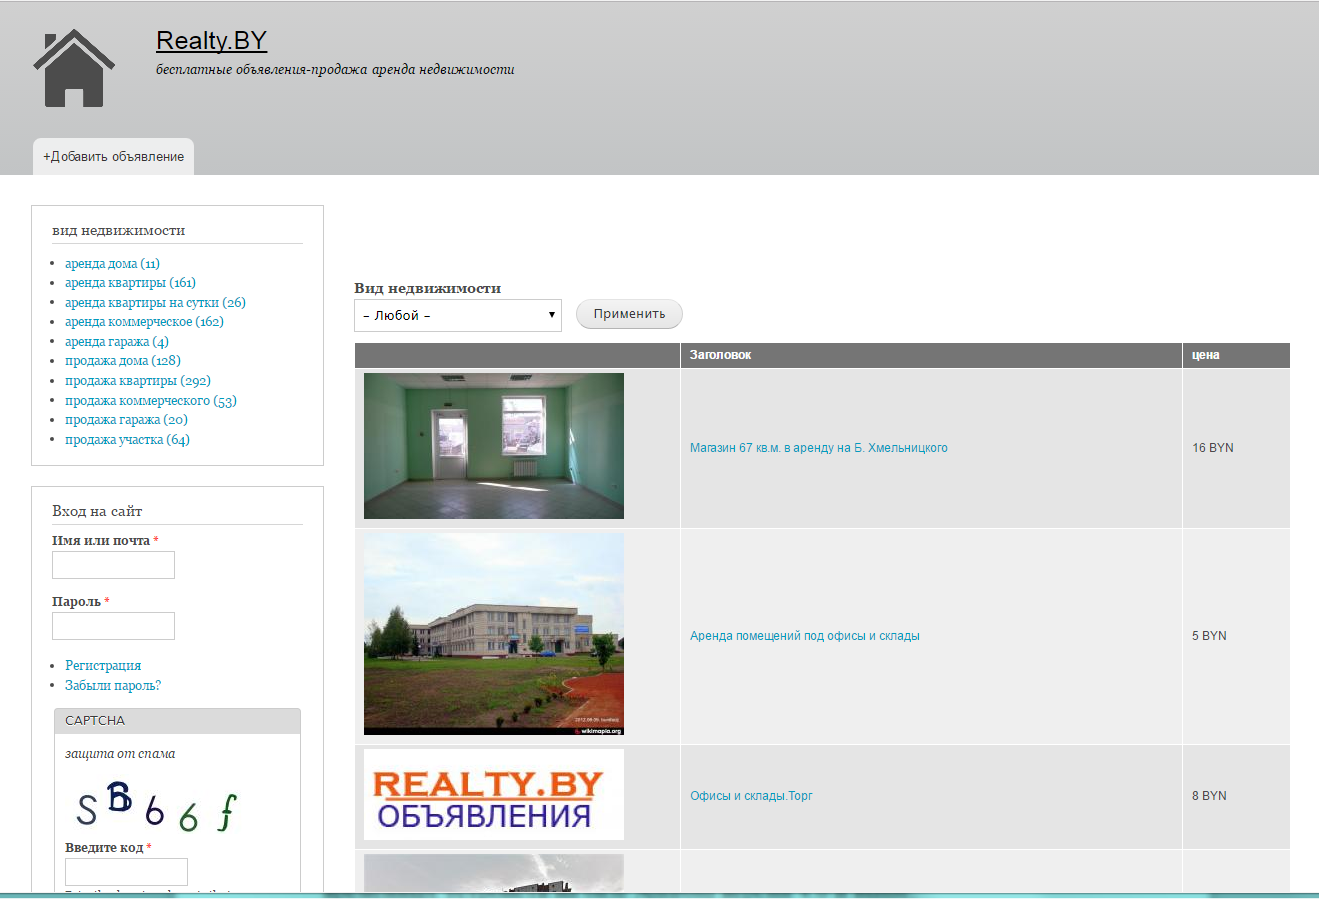
\includegraphics[scale=0.25]{realt1.png}
	\caption{ Главный страница программного средсва }
	\label{fig:arch_and_mod::realt1}
	\clearpage
\end{figure}

Реалт.бай это простой способ для размещения объявлений в сети. Веб-интерфейс простой в использовании, все объявления хранятся в базе данных.

Реалт.бай это портал, на котором собрана вся информация о жилой и коммерческой недвижимости в Беларуси. На сайте можно найти информа-цию по вопросам аренды квартир и комнат в Минске, продаже квартир.

Прежде чем добавить объявление, необходимо пройти процедуру регистрации на сайте. Операция по добавлению нового объявления выглядит следующим образом. Пользователю необходимо добавить описание, тему заголовка, цену,  добавить контактные данные. После этого будет размещено объявление.

\begin{figure}[!htb]
	\centering
	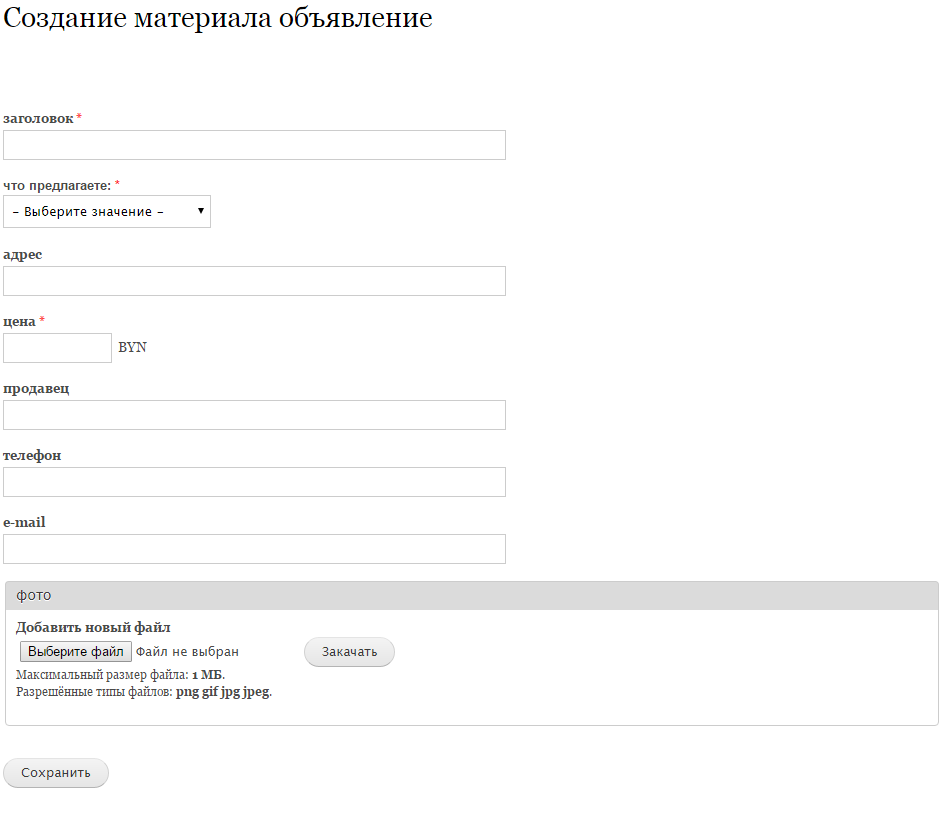
\includegraphics[scale=0.3]{realt2.png}
	\caption{ Добавление нового объявления }
	\label{fig:arch_and_mod::realt2}
	\clearpage
\end{figure}

Среди возможностей программного средства реалт.бай  можно выде-лить следующие достоинства:

\begin{itemize}
	\item понятный и простой интерфейс.
	\item возможность размещать объявление не только о продажи недвижимости.
	\item легкая обратная связь между клиентом и риелтором.
\end{itemize}

Помимо всех плюсов, стоит отметить несколько минусов данного программного средства:

\begin{itemize}
	\item только один критерий для поиска объявлений.
	\item нет возможности редактирования информации.
	\item большинство предложений уже не актуально.
\end{itemize}

Таким образом, это программное средство подходит в качестве простого приложения, решающее только частично описанные проблемы.

Квартирант.бай это программное средство, предоставляющее следующий перечень услуг:

\begin{itemize}
	\item аренда квартир;
	\item аренда комнат;
	\item аренда гостинец;
	\item продажа недвижимости;
\end{itemize}

\begin{figure}[!htb]
	\centering
	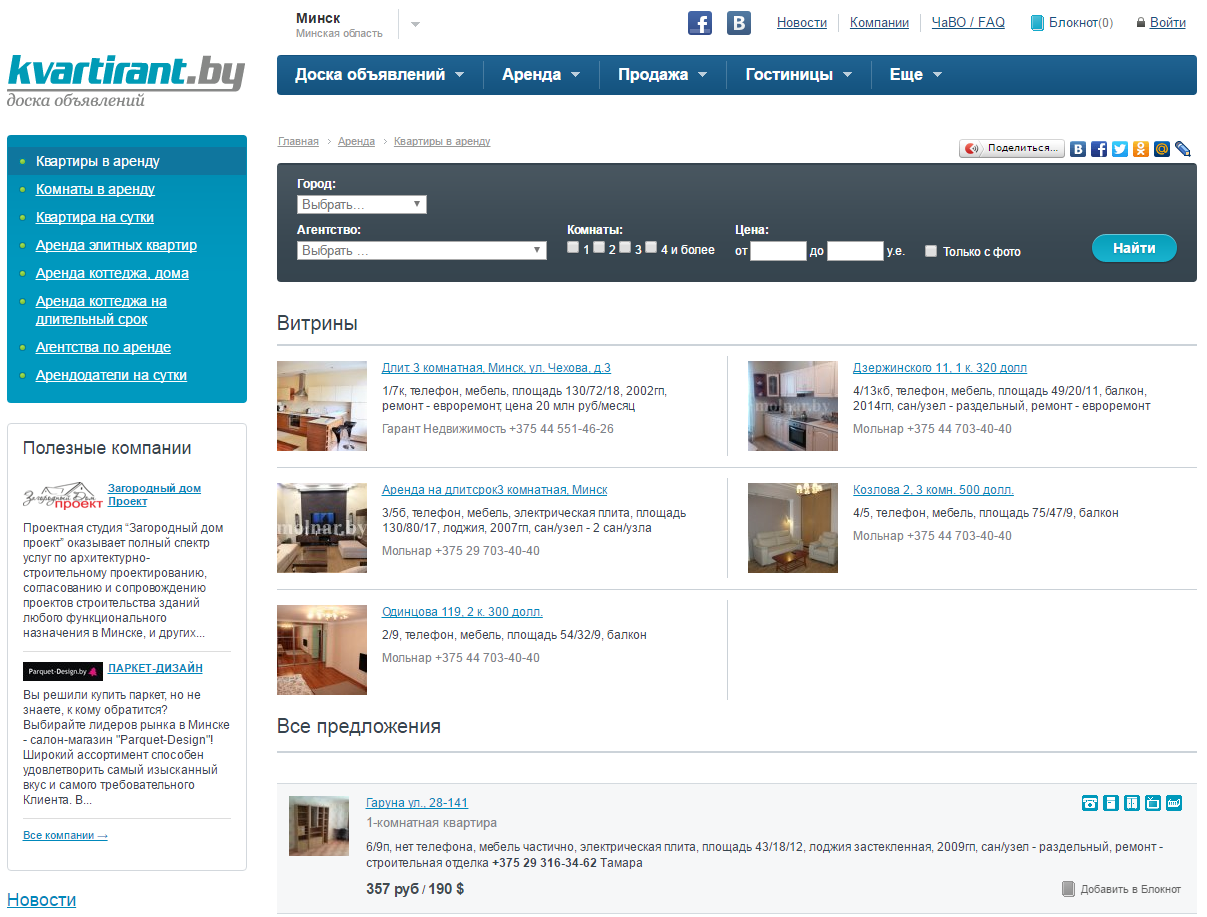
\includegraphics[scale=0.3]{kv_1.png}
	\caption{ Доска объявлений }
	\label{fig:arch_and_mod::lexer_flow}
	\clearpage
\end{figure}

Проект квартирант.бай стартовал в 2004 году как специализированный сайт по аренде всех видов недвижимости. Доска объявлений портала Квартирант.бай является популярной площадкой для бронирования гостинец, покупки недвижимости, аренды квартир.

Среди возможностей программного средства y можно выделить следующие достоинства:

\begin{itemize}
	\item понятный интерфейс;
	\item легкая обратная связь между клиентом и риелтором;
	\item возможность размещать объявление не только о продажи недвижимости;
\end{itemize}

Помимо всех плюсов, стоит отметить несколько минусов данного программного средства:

\begin{itemize}
	\item реклама;
	\item нет возможности редактирования информации;
	\item нет возможности оставить отзывы;
\end{itemize}

Таким образом, это программное средство подходит в качестве приложения, решающе не все описанные проблемы.

% \begin{explanation}

Программное средство оказывает услуги в сфере недвижимости. Продажа, покупка, обмен, разъезд, аренда комнат, квартир, коттеджей, дач, земельных участков, коммерческой недвижимости. Приватизация, утверждение перепланировок, вывод в нежилой фонд, консервация и другое.

\begin{figure}[!htb]
	\centering
	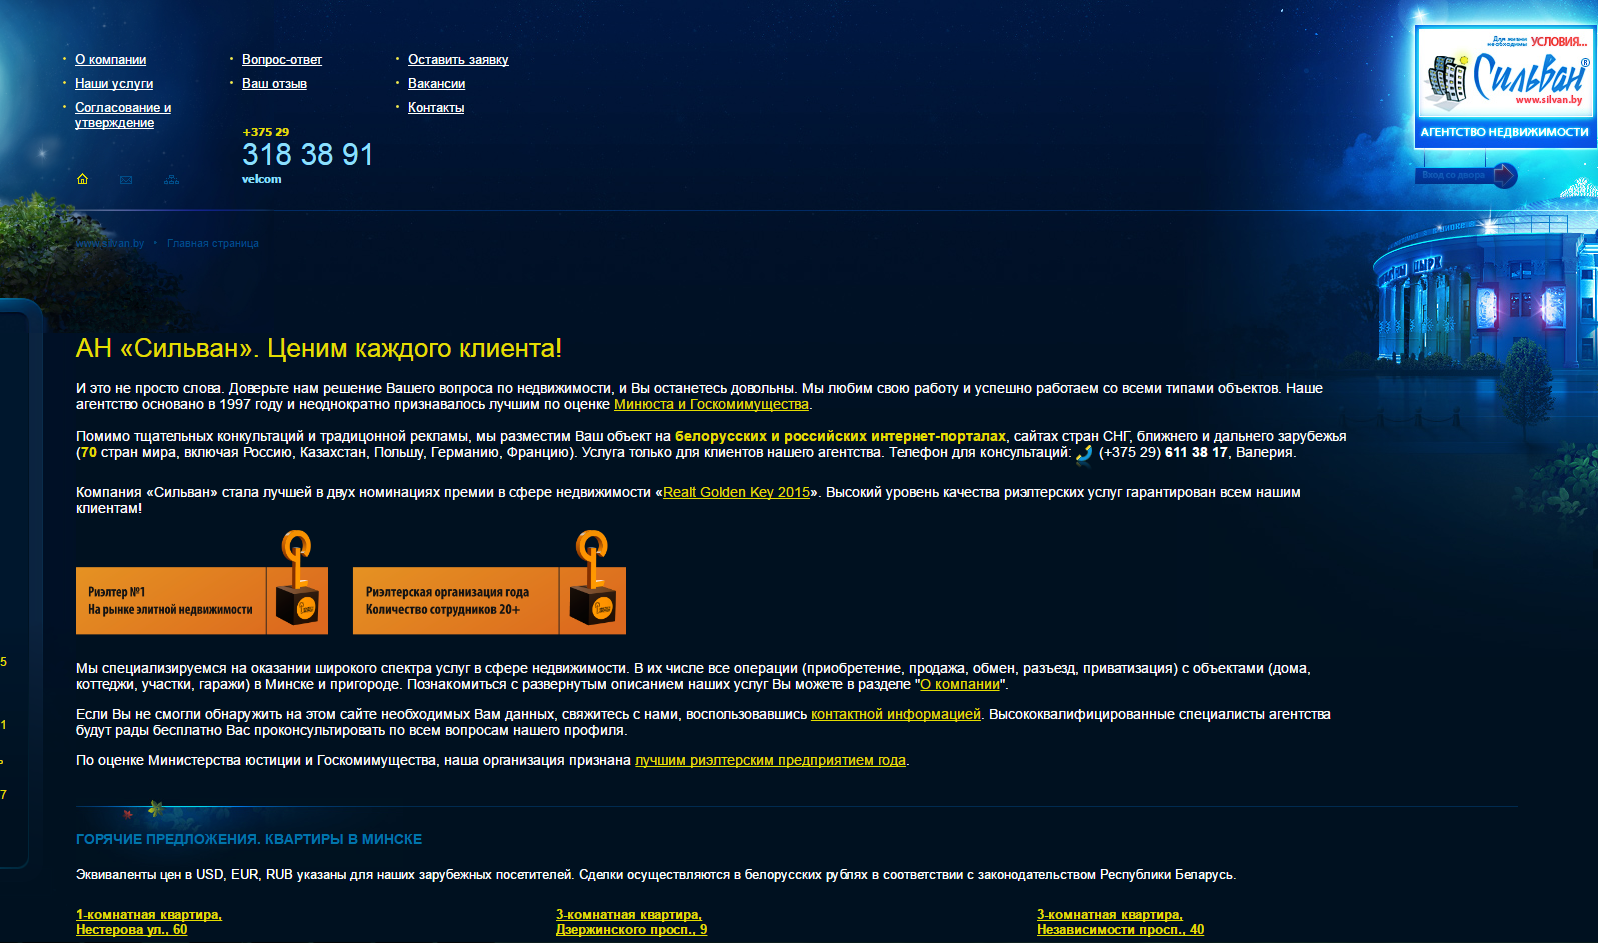
\includegraphics[scale=0.3]{sl_1.png}
	\caption{ Главная форма программного средства}
	\label{fig:arch_and_mod::lexer_flow}
	\clearpage
\end{figure}

Среди возможностей программного средства y можно выделить следующие достоинства:

\begin{itemize}
	\item обратная связь между клиентом и риелтором;
	\item возможность поиска по различным критериям;
\end{itemize}

Стоит отметить минусы данного программного средства:

\begin{itemize}
	\item яркий дизайн;
	\item нет пользователей как таковых
	\item нет возможности редактирования информации;
	\item нет возможности оставить отзывы;
	\item нет возможности добавить объявление;
	\item все операции делаются в ручную, клиент должен обратиться в офис компании;
\end{itemize}

Таким образом, данное программное средство не решает  множество описанных проблемы. Программное средство представляет из себя частный случай для риэлтерской компании.

\subsection{Постановка задачи}
В результате выполнения дипломного проекта должно быть разработано программное средство для продажи квартир через веб-интерфейс. 

Необходимо выполнить следующие задачи:

\begin{itemize}
	\item изучить и улучшить знания в web разработке приложения;
	\item ознакомиться с многопоточными приложениями и особенностями платформы java;
	\item разработать программное средство для продажи квартир; 
	\item разработать масштабируемое приложение, чтобы была возможность в будущем реализовывать дополнительный функционал;
\end{itemize}

Программное средство должно иметь два уровня доступа: администратор и пользователь. Пользователь может иметь доступ к своей учетной записи для добавления, поиска, редактирования своих объявлений. Администратор должен иметь возможность настраивать веб-интерфейс и управлять зарегистрированными пользователями.

Должны быть реализованы следующие ключевые функции:

\begin{itemize}
	\item создание учетной записи пользователя;
	\item восстановление учетной записи пользователя;
	\item добавление объявления;
	\item редактирование объявления;
	\item удаления  объявления;
	\item добавление фотографий;
	\item поиск объявления по множеству критериев;
	\item возможность оставить отзыв;
\end{itemize}

В процессе дипломного проектирования необходимо разработать приложение, которое будет решать все поставленные задачи и основные функции.
